\chapter*{Introducción}
\label{intro}

\epigraph{La vida sin pruebas y desafíos no sería provechosa, sino. ¿Como aprenderíamos?}%
{\textbf{Josue Alvarez. Guatemala }}

\par Debido al gran número de datos generados por los experimentos biológicos actuales, una nueva clase de híbridos ha surgido entre informáticos y biólogos. Los mismos se encargan de desarrollar métodos y programas para el análisis masivo de la información biológica. Dentro de esta línea, la \emph{Bioinformática} es considerada una de las disciplinas con mayor índice de expansión y crecimiento en la actualidad. 

\par No se puede abordar la Bioinformática sin describir inicialmente algunos conceptos elementales de la \emph{Biología}. En realidad son los biólogos y los bioquímicos quienes hicieron su primer acercamiento a la tecnología computacional como elemento fundamental para su trabajo diario. La tecnología proporciona un elemento teórico y las herramientas prácticas necesarias para que los científicos puedan explorar, analizar y establecer conclusiones al respecto.

\section*{La Biología}

\par \emph{La Biología} es aquella ciencia que estudia a los seres vivos, ya sean estos animales, plantas o seres humanos. Principalmente se preocupa de los procesos vitales de cada ser, tales como su nacimiento, desarrollo, muerte y procreación. Por lo que estudia el ciclo completo de los mismos\cite{curtis}. La palabra como tal, proviene del griego, \emph{bios} (vida) y \emph{logos} (estudio). Es decir, \emph{Estudio de la vida}.

\par En particular, una de las áreas de aplicación de la Biología es la Virología, la cual estudia la acción de los virus y cómo pueden ser aplicados ciertos fármacos para su tratamiento.

\par Todos los seres vivos existentes sintetizan proteínas. De hecho, los tipos celulares (procariotas o eucariotas) están determinados por los tipos de proteínas que cada célula puede sintetizar. Por este motivo el material genético debe controlar los tipos y cantidades de proteínas que sintetiza una célula. Prácticamente todos los procesos biológicos dependen de la presencia o la actividad de proteínas. Dentro de las diversas funciones que desempeñan, se pueden mencionar las siguientes: función defensiva (crean los anticuerpos y regulan factores contra agentes extraños o infecciones), función reguladora (colaboran en la regulación de la actividad de las células, por ejemplo en la división celular), función estructural o de construcción (forman parte de las estructuras corporales suministrando el material necesario para el crecimiento y la reparación de tejidos y órganos del cuerpo), función energética (cuando el aporte de hidratos de carbono y grasas resulta insuficiente para cubrir las necesidades energéticas, las proteínas se emplean como combustible energético),  entre otras. 

\par Las \emph{proteínas}, también denominadas polipéptidos, están constituidas por cadenas de un surtido de sólo 20 \emph{aminoácidos}. A su vez, cada aminoácido se encuentra conformado por una sucesión de tres \emph{nucleótidos} consecutivos, los cuales se los denominan \emph{codón} o \emph{triplete}, y codifican a un determinado aminoácido. A pesar de ello, existen aminoácidos que son codificados por más de una combinación de codones, a los cuales se los conoce como \emph{codones sinónimos}. Desde una perspectiva computacional, esta secuencia de nucleótidos se trata de una cadena de caracteres pertenecientes al alfabeto de los 4 nucleótidos del \emph{DNA}(Ácido Desoxirribonucleico) conocidos como \emph{A}denina, \emph{C}itosina, \emph{G}uanina y \emph{T}imina. 

\par El nexo entre el DNA que se encuentra en el núcleo celular y las proteínas, que se encuentra en los ribosomas(citoplasma), lo conforma el RNA(Ácido Ribonucleico), aunque el mismo puede ser funcional por sí mismo (figura~\ref{fig}). Este flujo de la información que lleva a la producción de proteínas se denomina \emph{Dogma Central de la Biología}. 

\begin{figure}[h!]
    \centering
    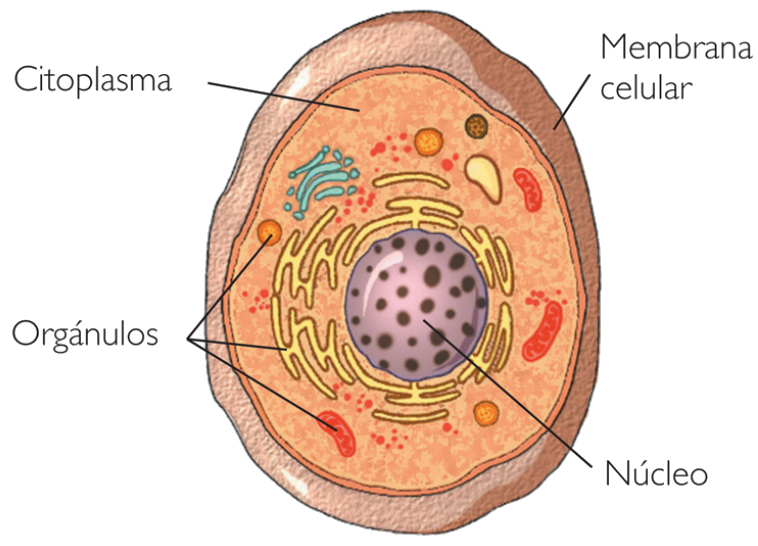
\includegraphics[scale=0.2]{image/celula.png}
    \caption{Estructura de un célula [1].}    
    \label{fig} 
\end{figure}    

\vskip 1cm
\par Básicamente, el DNA transfiere la información al RNA, el cual controla directamente la síntesis de proteínas. Este flujo es unidireccional, aunque existen excepciones. En este proceso entran en juego dos etapas importantes conocidas como \emph{transcripción} y \emph{traducción}. La transcripción es el proceso mediante el cual el RNA es sintetizado a partir de un molde de DNA, esto significa, que la información del DNA es reescrita, pero básicamente en el mismo lenguaje de nucleótidos. Por otro lado, la traducción es el proceso por el cual el RNA controla la síntesis de proteínas. En términos generales la información en el lenguaje de nucleótidos es traducida al lenguaje de aminoácidos\cite{genetica}. El proceso mencionado anteriormente se exhibe gráficamente en la figura~\ref{figIntro}.

\begin{figure}[h!]
    \centering
    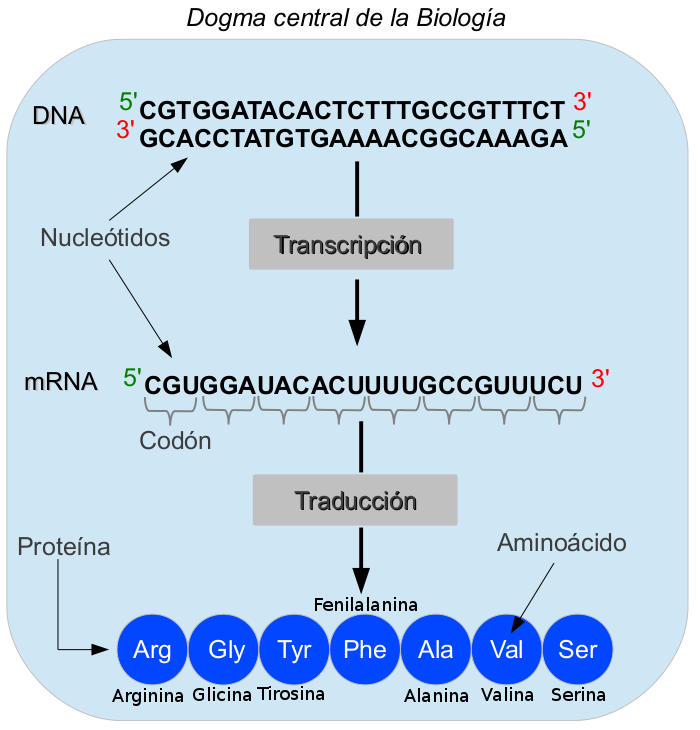
\includegraphics[scale=0.45]{image/resumen.png}
    \caption{Integrando conceptos iniciales [2].}
    \label{figIntro} 
\end{figure}    

\par Las secuencias mencionadas poseen diversos tamaños lo cual dificulta su procesamiento y análisis de forma manual. Las secuencias de proteínas contienen en promedio entre 100 y 5000 aminoácidos. Por otro lado, las secuencias de DNA son mucho más grandes que las de proteínas. Por ejemplo, el DNA de la bacteria E. Coli tiene 4.7 millones de nucleótidos y el del humano 3.3 billones.

\section*{La Bioinformática}
\par Si bien no existe una única definición, puede decirse que \emph{la Bioinformática} es la aplicación de las Ciencias de la Computación a la Biología Molecular. Este término hace referencia a campos de estudios interdisciplinarios muy vinculados, que requieren el uso o el desarrollo de diferentes técnicas que incluyen informática, matemática aplicada, estadística, Ciencias de la Computación, Inteligencia Artificial, Química y Bioquímica para solucionar problemas, analizar datos, o simular sistemas o mecanismos, todos ellos de índole biológica, y usualmente de nivel molecular. El núcleo principal de estas técnicas se encuentra en la utilización de recursos computacionales para solucionar o investigar problemas sobre escalas de tal magnitud que sobrepasan el discernimiento humano. 
\par Según la definición del Centro Nacional para la Información Biotecnológica (``National Center for Biotechnology Information'', NCBI por sus siglas en Inglés, 2001):
\begin{center}
\emph{``La Bioinformática es un campo de la ciencia en el cual confluyen varias disciplinas tales como: biología, computación y tecnología de la información. El fin último de este campo es facilitar el descubrimiento de nuevas ideas biológicas así como crear perspectivas globales a partir de las cuales se puedan discernir principios unificadores en biología.''}
\end{center}

\par Históricamente, el uso de las computadoras para resolver cuestiones biológicas comenzó con el desarrollo de algoritmos y su aplicación en el entendimiento de las interacciones de los procesos biológicos entre diversos organismos. La Biología Molecular es una ciencia rica en datos que crecen a tasas exponenciales\cite{NCBI}. Sin embargo, desde la perspectiva computacional la característica clave de los datos biológicos no es tanto su volumen sino su diversidad, heterogeneidad y dispersión, lo que impide o dificulta la explotación integrada de esta información.
\textbf{Los ``grandes volúmenes de datos'' se suelen citar como una de las características mas relevantes de la Bioinformática debido a sus tasas exponenciales de crecimiento.} Este crecimiento se debe en buena medida al desarrollo de nuevas tecnologías, permitiendo pasar del estudio de genes individuales a genomas completos y ahora a la interacción entre organismos.

\section*{\remo}
\par Luego de mencionar brevemente algunos conceptos importantes a continuación se presenta el trabajo titulado: \emph{``Estudio de la relación de divergencia en el uso de codones sinónimos entre virus-huésped y presencia de microRNA''}. El mismo tiene como principal objetivo contrastar una teoría postulada y encomendada por el Dr. Roberto Daniel Rabinovich\footnote{Miembro del Instituto Biomédico en Retrovirus y SIDA-INBIRS e investigador del Consejo Nacional de Investigaciones Científicas y Técnicas (CONICET), Buenos Aires, Argentina.}, que involucra principalmente la molécula de RNA. Dicho estudio surge como propuesta de la fundación FuDePAN\footnote{Fundación para el Desarrollo de la Programación en Ácidos Nucleicos, Córdoba, Argentina. \url{http://www.fudepan.org.ar/}}.

\par Se desea estudiar si la divergencia en el uso de codones sinónimos entre virus y huésped contribuye a disminuir la interferencia de los microRNA ($_m$$_i$RNA) en la expresión de los RNA mensajeros($_m$RNA) de origen viral. Los $_m$$_i$RNA son pequeñas moléculas codificadas en el DNA de las distintas especies que regulan la expresión de una gran fracción de las proteínas\footnote{Los $_m$$_i$RNA reconocen secuencias parcialmente complementarias en un $_m$RNA correspondiente, dando como resultando la inhibición de la traducción de dicho $m$RNA.}. Un $_m$RNA es un tipo particular de ácido ribonucleico monocatenario que contiene la información genética procedente del DNA(bicatenario) para utilizarse en la síntesis de proteínas. De esa manera se contribuirá a comprender mejor la relación virus-huésped y la evolución viral. Estos estudios tienen también una importancia potencial en la comprensión de la patogenia viral y en el desarrollo de herramientas terapéuticas como la terapia génica.

\par Para lograr tal objetivo se plantea desarrollar un software que, dadas ciertas secuencias de $_m$RNA y secuencias de $_m$$_i$RNA, permita determinar si la divergencia en el uso de codones sinónimos entre virus y huésped contribuye a disminuir la interferencia de los $_m$$_i$RNA en la expresión de los $_m$RNA de origen viral.

\par Dada la gran cantidad de datos a manipular y el tamaño de las secuencias, se requiere de un gran número de pequeños cálculos y comparaciones lo cual demanda un alto poder de cómputo. Por otro lado, para tener soporte de la ejecución distribuida se plantea utilizar el framework \emph{FuD}\footnote{FuDePAN Ubiquitous Distribution}\cite{clus09} sin tener que desarrollar específicamente esta funcionalidad y sin perder de vista el problema original.

\par Algunos motivaciones que llevaron a tomar la decisión de realizar el presente proyecto refieren a la posibilidad de enfrentarse con un problema real, de índole biológico, manipulando datos muy complejos tales como secuencias de DNA, secuencias de virus, entre otras. Por otro lado, de cierto modo, 
estos estudios pueden servir para contribuir a la investigación de temas relacionados con el área de la salud.

\par En el resto del documento se empleará el término \textbf{R-emo} o \remo para referirse al software desarrollado como solución planteada.

\section*{Estructura del Documento}
El documento esta compuesto por 8 capítulos, los cuales se detallan brevemente a continuación. 
\begin{itemize}
    \item \emph{Capítulo 1: La Biología,} describe los conceptos biológicos elementales necesarios para comprender el trabajo realizado. Algunos temas específicos quedan fuera del alcance de este documento, debido a la complejidad de los mismos, aunque no dejan de ser importantes.
    \item \emph{Capítulo 2: Descripción del Problema,} introduce el problema a resolver con una descripción general. 
    \item \emph{Capítulo 3: Metodología de Trabajo,} abarca la metodología de desarrollo seleccionada, detallando el modelo clásico y algunas consideraciones que se tuvieron en cuenta. Se describen las prácticas de software y herramientas empleadas.    
    \item \emph{Capítulo 4: Elicitación y Análisis de Requerimientos,} se describe brevemente la elicitación de requisitos y el análisis de los mismos, enunciando el estudio de las herramientas necesarias y búsqueda de datos mínimos.
    \item \emph{Capítulo 5: Diseño,} se menciona la arquitectura global de \remo y algunas consideraciones de diseño. 
    \item \emph{Capítulo 6: Implementación,} abarca detalles de implementación, representación de datos biológicos, el framework empleado para distribuir el trabajo, métricas de código, etcétera.
    \item \emph{Capítulo 7: Experimentación y Testing,} corresponde a las pruebas de \remo y las herramientas empleadas para tal fin.
    \item \emph{Capítulo 8: Conclusiones del Trabajo,} se detalla la conclusión del presente trabajo, los resultados, aportes y futuros desarrollos.    
\end{itemize}
A continuación de describe el presente trabajo.